% !TeX root = ../libro.tex
% !TeX encoding = utf8

\chapter{Guía de uso del programa}\label{ap:apendice2}

En este capítulo se explicará brevemente cómo utilizar el programa. Aun así, la interfaz del programa se ha intentado diseñar lo más sencilla y clara posible, mostrando adicionalmente cuadros de texto si se mantiene el ratón sobre ciertos elementos.\\
\\Si sólo quiere hacer uso del programa ``procesador'', ejecute el comando:
\begin{center}
 make read FILE=<archivo>
\end{center}
pero desde el directorio ``processor'. Esta acción devolverá la traducción de ``<archivo>'' al fichero ``../shaders/functions.s'' y la salida de error en ``../error.log''.\\
\\Si queremos utilizar el programa completo, primero instalaremos el programa tal y como se indica en el apéndice de \textbf{Instalación del software}. Una vez instalado, se abrirá siempre con el comando ``make'', ``make execute'' o equivalentemente ``./bin/program''. Teniendo abierto el programa se mostrará siempre la última parametrización compilada con éxito. En el lateral izquierdo aparecerá un elemento de la interfaz, el menú, donde se podrá modificar:
\begin{itemize}
	\item Parametrización:
	\begin{itemize}
		\item Seleccionar una parametrización ya existente, crearla o compilarla. También se podrá editar la actual, en cuyo caso aparecerá una ventana de edición de la propia interfaz. Dicha ventana también aparecerá en caso de que hayan errores léxicos, sintácticos o semánticos en la parametrización, con la salida del error desplegada. Como ejemplos se aportarán parametrizaciones de una gran variedad de superficies, ubicadas en el directorio ``manifolds''.
		\item Cambiar el tamaño de la malla de partida, confirmando con la tecla ``Enter''.
		\item Visualizar la ventana con los parámetros temporales, con un tick que indica si está activa la ventana o no. Estará semi-visible si la superficie no tiene parámetros temporales. Dicha ventana mostrará los parámetros temporales en orden, permitiendo moverlos manualmente o generar una animación:
		\begin{itemize}
			\item Sin: movimiento sinusoidal entre el valor $0$ y $1$. Ideal para animaciones oscilantes.
			\item Lineal: movimiento lineal del valor $0$ al $1$, volviendo instantáneamente al $0$. Utilizado para movimientos lineales respecto al tiempo, que junto con el uso de funciones periódicas se puede generar la sensación de movimiento infinito (como los ejemplos wavesX.in).
		\end{itemize}
	\end{itemize}
	\item Visualización del objeto:
	\begin{itemize}
		\item Invertir normales (si no se quiere modificar la parametrización).
		\item Visualizar en modo malla (``Polygon mode'').
		\item Activar/desactivar la auto-rotación (rotación orbital entorno al punto hacia el que mira la cámara).
		\item Ver los vectores tangentes, bitangentes y normales a los puntos (ya sean los de la malla inicial o de todos los generados).
		\item Cambiar modo del color de la superficie, ya sea el color base, la curvatura de Gauss, el área diferencial, la altura o los puntos críticos de ésta vista como función de Morse. Una vez seleccionado un modo, aparecerán coeficientes que permitirán ajustar correctamente la visualización a la superficie actual.
	\end{itemize}
	\item Opciones del teselado:
	\begin{itemize}
		\item Desactivar/activar el teselado.
		\item Indicar la precisión a la que se desea llegar con el teselado.
		\item Opciones avanzadas: modificar aquellos coeficientes específicos del teselado, como el tipo de mejora de rendimiento a usar (``improve'' normal o específica), la distancia de teselado, el umbral para detectar bordes y el exponente aplicado a la curvatura de Gauss. Todos ellos se inician con un valor por defecto.
	\end{itemize}
	\item Iluminación: es posible cambiar los coeficientes del modelo de iluminación ``Phong'' y ver el vector de dirección de la luz actualmente. La luz no es direccional, el vector indica la dirección de la luz con respecto al origen $(0,0)$.
	\item Estadísticas: muestra los fotogramas por segundo y la latencia medias, junto con el número de primitivas generadas tras la fase del geometry shader (después del tessellation shader). Permite además grabar los datos y los almacena de manera automática tras 22 segundos (antes si pulsamos ``Stop'' y seguidamente ``Save info'') en un fichero en el directorio raíz, con nombre dependiente de la parametrización y configuración actual.
\end{itemize}

\begin{figure}[h]
  	\centering
  	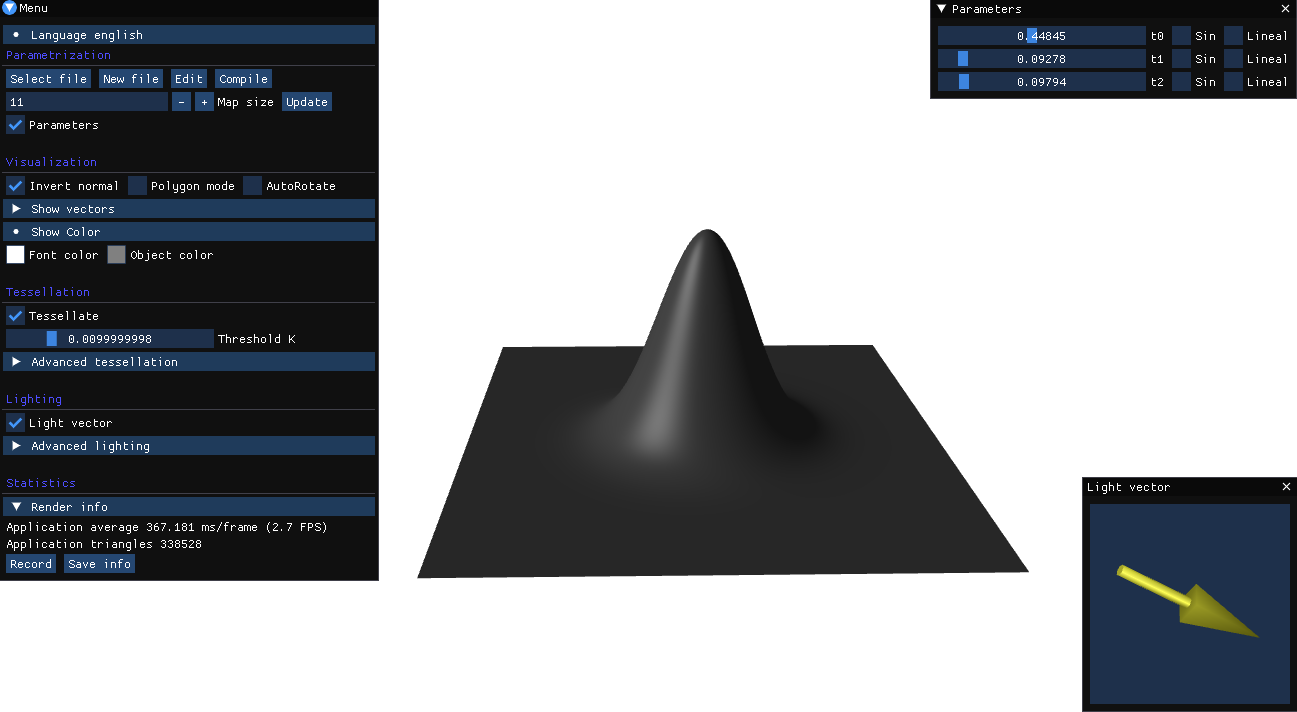
\includegraphics[width=0.9\textwidth]{interfaz1}
  	\caption{Ventanas iniciales.}
  	\label{fig:interfaz1}
\end{figure}
\newpage
\begin{figure}[h]
  	\centering
  	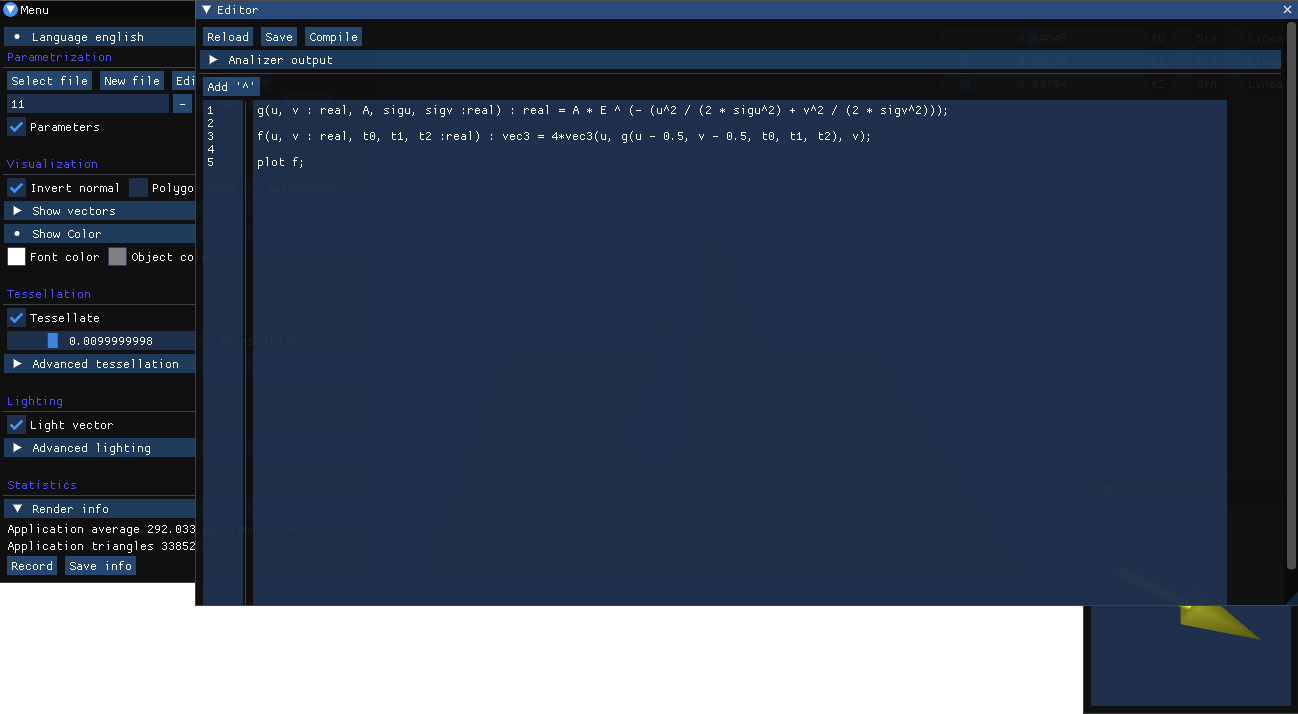
\includegraphics[width=0.9\textwidth]{interfaz2}
  	\caption{Ventana de edición de código.}
  	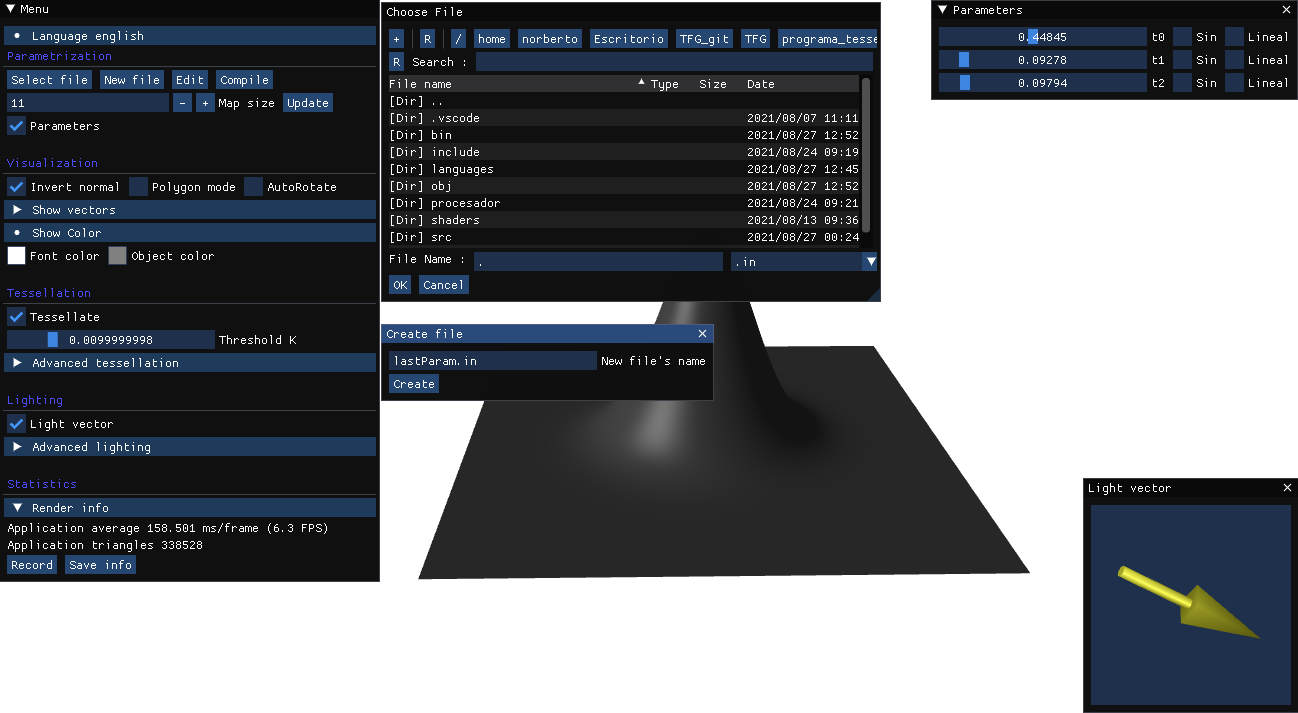
\includegraphics[width=0.9\textwidth]{interfaz3}
  	\caption{Ventanas de selección y creación de archivos.}
  	\label{fig:interfaz23}
\end{figure}
\newpage
Para mayor comodidad, se han incorporado atajos de teclado para ciertas acciones:
\begin{itemize}
	\item 'LCtrl' + 'R': activa/desactiva el modo de rotación automática.
	\item 'LCtrl' + 'P': cambia entre los modos de visualización malla y relleno.
	\item 'LCtrl' + 'N': activa/desactiva la visualización de normales.
	\item 'LCtrl' + 'L': ejecuta el ``procesador'' y compila los shaders.
\end{itemize}

Además, existen varios controles del ratón para manejar la cámara:
\begin{itemize}
	\item Botón izquierdo: si se mantiene pulsado y arrastramos, la cámara realizará una traslación en la dirección contraria.
	\item Botón derecho: si se mantiene pulsado y arrastramos, la cámara realizará una rotación (cámara orbital) en la dirección contraria.
	\item Rueda: controla el zoom.
	\item Botón de la rueda: reinicia la posición de la cámara.
\end{itemize}

\endinput
%------------------------------------------------------------------------------------
% FIN DEL APÉNDICE. 
%------------------------------------------------------------------------------------
